\documentclass{standalone}
\usepackage{xcolor}
\usepackage{tikz}
\usetikzlibrary{positioning, shapes.multipart, calc, graphs, graphs.standard}
\begin{document}
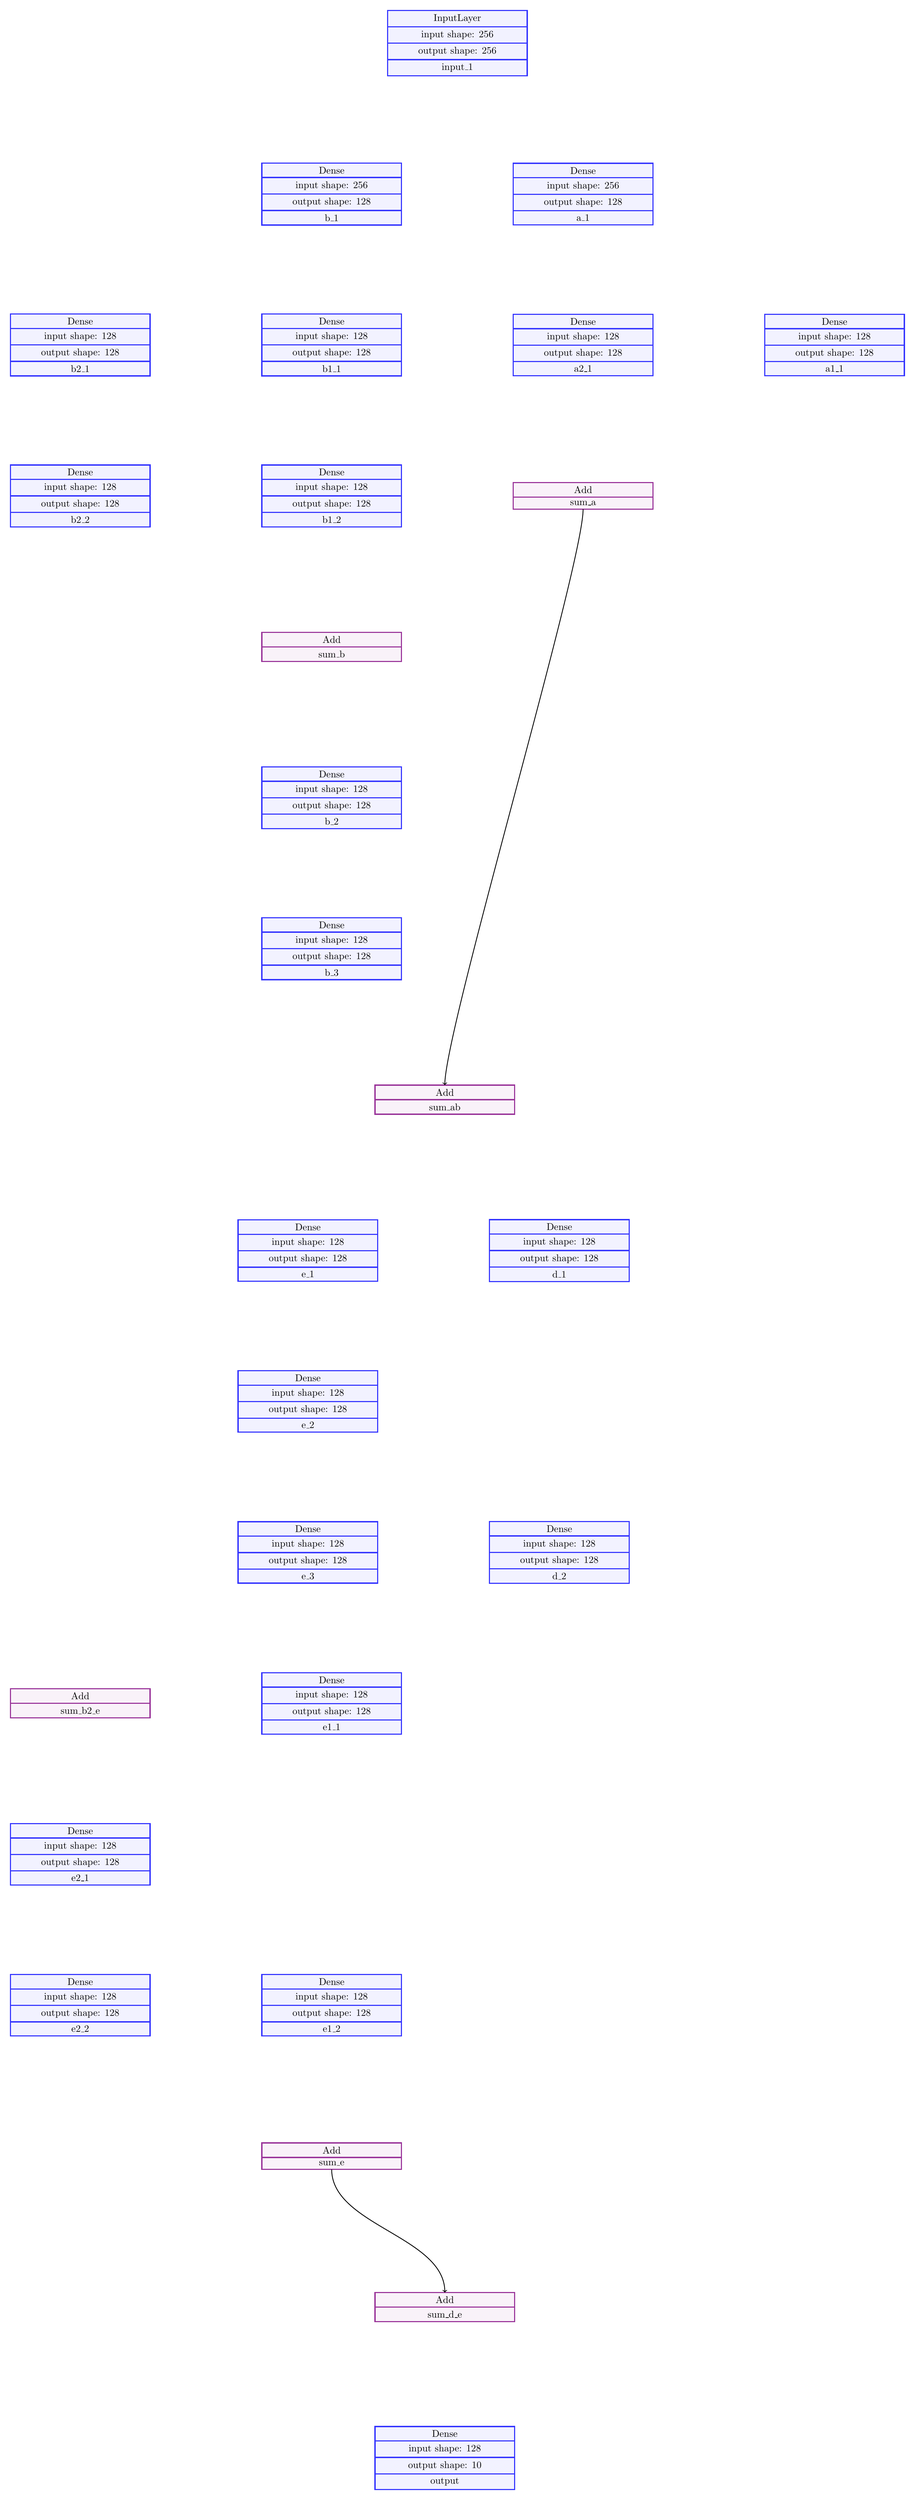
\begin{tikzpicture}
% style: defaultEdge
\tikzstyle{defaultEdge}=[thick,out=-90,in=90,out distance=2cm,in distance=2cm]
% style: defaultLabel
\tikzstyle{defaultLabel}=[auto,pos=0.65]
% style: OperationLayer_style
\tikzstyle{OperationLayer_style}=[rectangle split,rectangle split ignore empty parts,very thick,rectangle split parts=5,draw=violet!80,fill=violet!5,minimum width=5cm,outer sep=0cm]
% style: UtilityLayer_style
\tikzstyle{UtilityLayer_style}=[rectangle split,rectangle split ignore empty parts,very thick,rectangle split parts=5,draw=gray!80,fill=gray!5,minimum width=5cm,outer sep=0cm]
% style: TrainableLayer_style
\tikzstyle{TrainableLayer_style}=[rectangle split,rectangle split ignore empty parts,very thick,rectangle split parts=5,draw=blue!80,fill=blue!5,minimum width=5cm,outer sep=0cm]

% node: input_1
\node[TrainableLayer_style] (input_1) at (16.2, 87.3)
    {
    \nodepart{one}{InputLayer}
    \nodepart{two}{input shape: 256}
    \nodepart{three}{output shape: 256}
    \nodepart{four}{input\_1}};

% node: b_1
\node[TrainableLayer_style] (b_1) at (11.7, 81.9)
    {
    \nodepart{one}{Dense}
    \nodepart{two}{input shape: 256}
    \nodepart{three}{output shape: 128}
    \nodepart{four}{b\_1}};

% node: b1_1
\node[TrainableLayer_style] (b1_1) at (11.7, 76.5)
    {
    \nodepart{one}{Dense}
    \nodepart{two}{input shape: 128}
    \nodepart{three}{output shape: 128}
    \nodepart{four}{b1\_1}};

% node: b2_1
\node[TrainableLayer_style] (b2_1) at (2.7, 76.5)
    {
    \nodepart{one}{Dense}
    \nodepart{two}{input shape: 128}
    \nodepart{three}{output shape: 128}
    \nodepart{four}{b2\_1}};

% node: b1_2
\node[TrainableLayer_style] (b1_2) at (11.7, 71.1)
    {
    \nodepart{one}{Dense}
    \nodepart{two}{input shape: 128}
    \nodepart{three}{output shape: 128}
    \nodepart{four}{b1\_2}};

% node: b2_2
\node[TrainableLayer_style] (b2_2) at (2.7, 71.1)
    {
    \nodepart{one}{Dense}
    \nodepart{two}{input shape: 128}
    \nodepart{three}{output shape: 128}
    \nodepart{four}{b2\_2}};

% node: sum_b
\node[OperationLayer_style] (sum_b) at (11.7, 65.7)
    {
    \nodepart{one}{Add}
    \nodepart{two}{sum\_b}};

% node: a_1
\node[TrainableLayer_style] (a_1) at (20.7, 81.9)
    {
    \nodepart{one}{Dense}
    \nodepart{two}{input shape: 256}
    \nodepart{three}{output shape: 128}
    \nodepart{four}{a\_1}};

% node: b_2
\node[TrainableLayer_style] (b_2) at (11.7, 60.3)
    {
    \nodepart{one}{Dense}
    \nodepart{two}{input shape: 128}
    \nodepart{three}{output shape: 128}
    \nodepart{four}{b\_2}};

% node: a1_1
\node[TrainableLayer_style] (a1_1) at (29.7, 76.5)
    {
    \nodepart{one}{Dense}
    \nodepart{two}{input shape: 128}
    \nodepart{three}{output shape: 128}
    \nodepart{four}{a1\_1}};

% node: a2_1
\node[TrainableLayer_style] (a2_1) at (20.7, 76.5)
    {
    \nodepart{one}{Dense}
    \nodepart{two}{input shape: 128}
    \nodepart{three}{output shape: 128}
    \nodepart{four}{a2\_1}};

% node: b_3
\node[TrainableLayer_style] (b_3) at (11.7, 54.9)
    {
    \nodepart{one}{Dense}
    \nodepart{two}{input shape: 128}
    \nodepart{three}{output shape: 128}
    \nodepart{four}{b\_3}};

% node: sum_a
\node[OperationLayer_style] (sum_a) at (20.7, 71.1)
    {
    \nodepart{one}{Add}
    \nodepart{two}{sum\_a}};

% node: sum_ab
\node[OperationLayer_style] (sum_ab) at (15.75, 49.5)
    {
    \nodepart{one}{Add}
    \nodepart{two}{sum\_ab}};

% node: e_1
\node[TrainableLayer_style] (e_1) at (10.85, 44.1)
    {
    \nodepart{one}{Dense}
    \nodepart{two}{input shape: 128}
    \nodepart{three}{output shape: 128}
    \nodepart{four}{e\_1}};

% node: e_2
\node[TrainableLayer_style] (e_2) at (10.85, 38.7)
    {
    \nodepart{one}{Dense}
    \nodepart{two}{input shape: 128}
    \nodepart{three}{output shape: 128}
    \nodepart{four}{e\_2}};

% node: e_3
\node[TrainableLayer_style] (e_3) at (10.85, 33.3)
    {
    \nodepart{one}{Dense}
    \nodepart{two}{input shape: 128}
    \nodepart{three}{output shape: 128}
    \nodepart{four}{e\_3}};

% node: sum_b2_e
\node[OperationLayer_style] (sum_b2_e) at (2.7, 27.9)
    {
    \nodepart{one}{Add}
    \nodepart{two}{sum\_b2\_e}};

% node: e1_1
\node[TrainableLayer_style] (e1_1) at (11.7, 27.9)
    {
    \nodepart{one}{Dense}
    \nodepart{two}{input shape: 128}
    \nodepart{three}{output shape: 128}
    \nodepart{four}{e1\_1}};

% node: e2_1
\node[TrainableLayer_style] (e2_1) at (2.7, 22.5)
    {
    \nodepart{one}{Dense}
    \nodepart{two}{input shape: 128}
    \nodepart{three}{output shape: 128}
    \nodepart{four}{e2\_1}};

% node: d_1
\node[TrainableLayer_style] (d_1) at (19.85, 44.1)
    {
    \nodepart{one}{Dense}
    \nodepart{two}{input shape: 128}
    \nodepart{three}{output shape: 128}
    \nodepart{four}{d\_1}};

% node: e1_2
\node[TrainableLayer_style] (e1_2) at (11.7, 17.1)
    {
    \nodepart{one}{Dense}
    \nodepart{two}{input shape: 128}
    \nodepart{three}{output shape: 128}
    \nodepart{four}{e1\_2}};

% node: e2_2
\node[TrainableLayer_style] (e2_2) at (2.7, 17.1)
    {
    \nodepart{one}{Dense}
    \nodepart{two}{input shape: 128}
    \nodepart{three}{output shape: 128}
    \nodepart{four}{e2\_2}};

% node: d_2
\node[TrainableLayer_style] (d_2) at (19.85, 33.3)
    {
    \nodepart{one}{Dense}
    \nodepart{two}{input shape: 128}
    \nodepart{three}{output shape: 128}
    \nodepart{four}{d\_2}};

% node: sum_e
\node[OperationLayer_style] (sum_e) at (11.7, 11.7)
    {
    \nodepart{one}{Add}
    \nodepart{two}{sum\_e}};

% node: sum_d_e
\node[OperationLayer_style] (sum_d_e) at (15.75, 6.3)
    {
    \nodepart{one}{Add}
    \nodepart{two}{sum\_d\_e}};

% node: output
\node[TrainableLayer_style] (output) at (15.75, 0.9)
    {
    \nodepart{one}{Dense}
    \nodepart{two}{input shape: 128}
    \nodepart{three}{output shape: 10}
    \nodepart{four}{output}};

% edge from sum_a to sum_ab
\draw[->, defaultEdge] (sum_a) to node [defaultLabel] {} (sum_ab);

% edge from sum_e to sum_d_e
\draw[->, defaultEdge] (sum_e) to node [defaultLabel] {} (sum_d_e);

\end{tikzpicture}\end{document}